\section{Introduction}

% \begin{figure}[h]
%   \centering
%   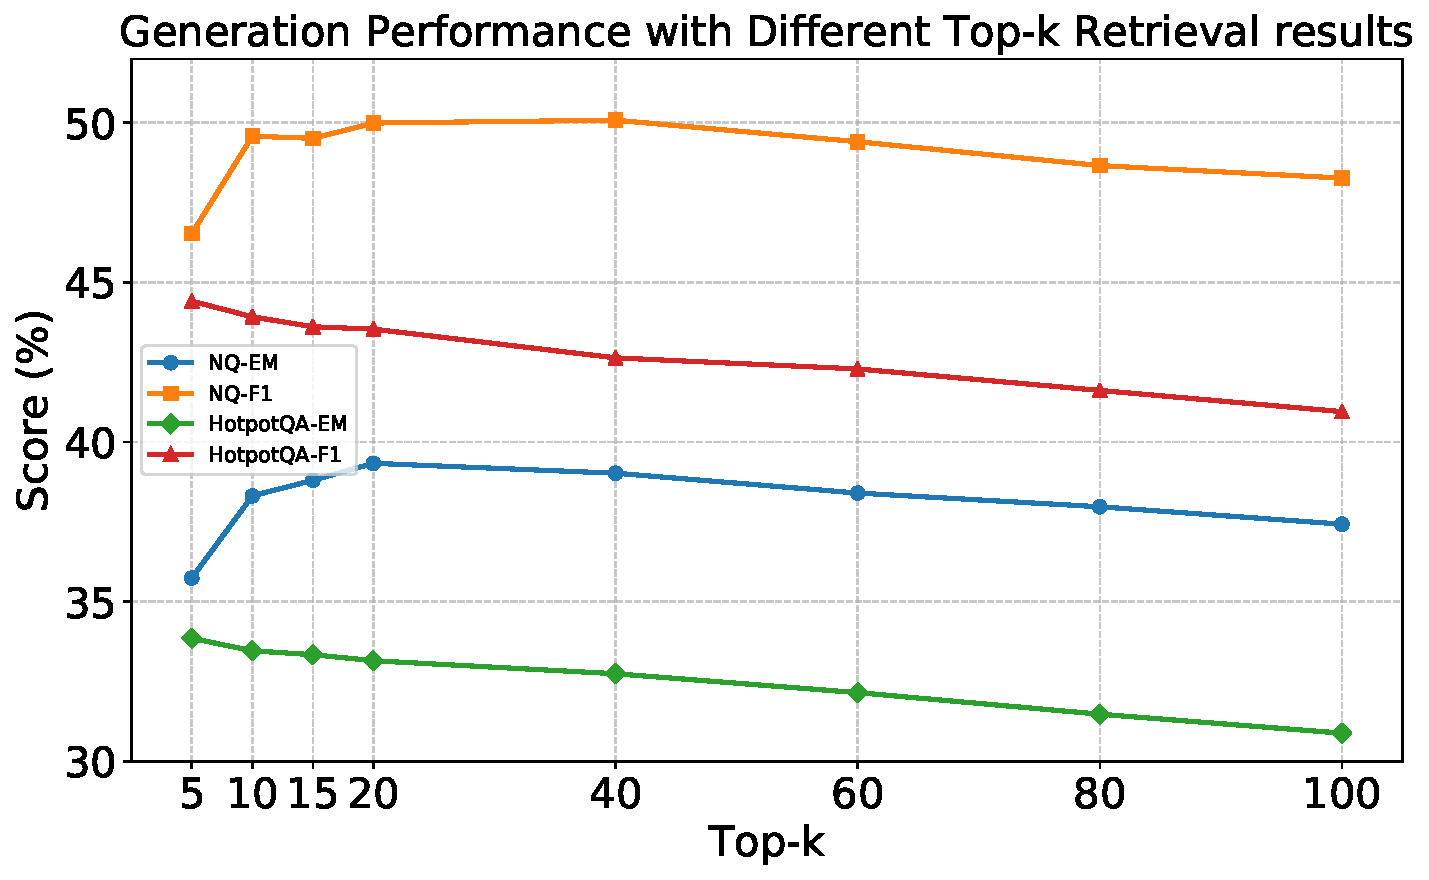
\includegraphics[width=\linewidth]{images/introduction.pdf}
%   \caption{Different answer generation performance (generator: Llama3.1-8B) directly with different top-$k$ retrieval results (retriever: BM25).}
%   \label{fig:original_ranked_answer}
% \end{figure}
\begin{figure}[h]
  \centering
  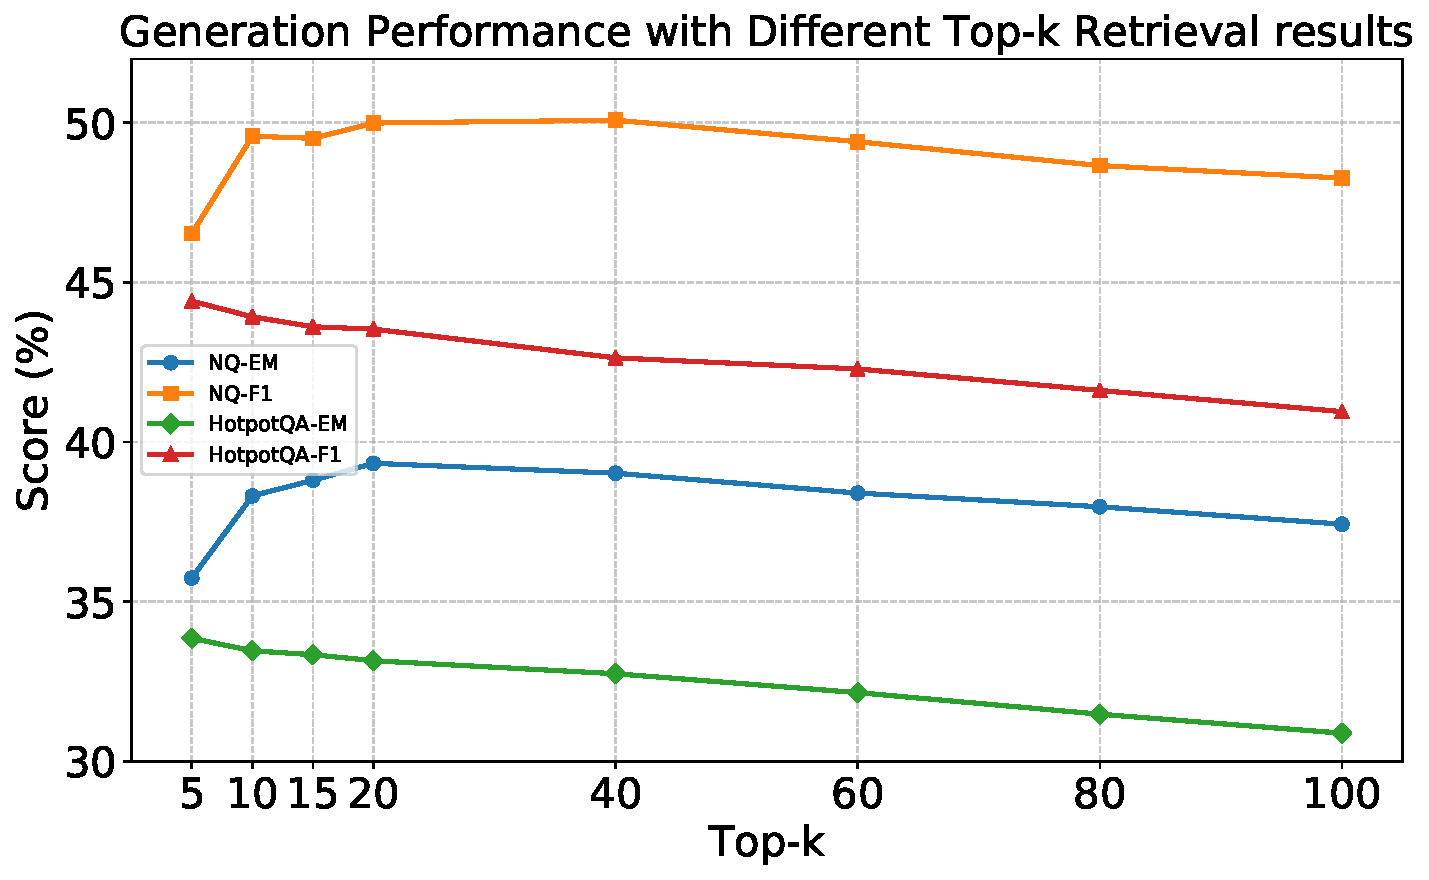
\includegraphics[width=\linewidth]{images/introduction.pdf}
  \caption{Different answer generation performance (generator: Llama-3.1-8B-Instruct) directly with different top-$k$ retrieval results (retriever: BM25).}
  \label{fig:original_ranked_answer}
\end{figure}
Retrieval-augmented generation (RAG) leverages retrieved information as external knowledge to empower large language models (LLMs) to answer questions. 
The criterion for measuring whether a result is helpful for RAG has shifted from relevance to utility \cite{shi2023replug,ke2024bridging,zhang2024large,zhang2024iterative}. 
Relevance typically focuses on the topical matching between a query and retrieved passages \cite{saracevic1988study, schamber1988relevance}. 
Utility, in contrast, emphasizes the usefulness of a passage in facilitating the generation of an accurate and comprehensive answer to the question \cite{zhang2025leveraging}. 
% Studies \cite{zhang2024large, zhang2024iterative} have also established this distinction, and 
Empirical results demonstrate that using retrieval results judged as having utility by LLMs in RAG can enhance the quality of subsequent answer generation \cite{zhang2024large,zhang2024iterative}. 



Due to the high computation cost, using LLMs for utility judgments usually takes 10 to 20 passages as context \cite{zhang2024large,zhang2024iterative}. This is insufficient for weaker retrievers that rank useful passages at lower positions, and when complex questions require many useful documents to generate comprehensive answers. 
Although it is promising to scale utility judgments to a large number of candidate passages for RAG, using LLMs to do so is cost-prohibitive. 
% Current studies \cite{zhang2024large, zhang2024iterative} typically restrict utility judgments to approximately 20 passages per query due to these constraints. 
% This limitation is particularly problematic for complex queries, such as multi-hop reasoning questions, which often require synthesizing information from numerous passages to generate a complete answer. A limit of around 20 passages may be insufficient for such cases. 
Therefore, we propose to distill the utility judgment capability of LLMs to smaller models that are efficient to do so.   
% a critical research direction is transferring the capability for utility judgment into smaller, more efficient models. 

In this paper, we focus on utility-based selection rather than ranking when distilling smaller models. There are two reasons: 1) \citet{ke2024bridging} find that for effective RAG, the ranking of input passages is less critical than effectively filtering out low-quality passages. 2) 
% While utility itself can be used to rank passages, 
The number of passages that should be selected for different questions can vary. As shown in Figure \ref{fig:original_ranked_answer}, the optimal number of passages used for simple questions (i.e., in NQ) and complex questions (i.e., in HotpotQA) is different. 
If we conduct utility ranking, 
% it needs to determine the number of passages to use for answer generation. 
a fixed threshold is usually used, which introduces a hyperparameter to tune and can be suboptimal. 
% inherently static and fails to adapt to the specific demands of individual queries. 
% As shown in Figure \ref{fig:original_ranked_answer}, the optimal passage number is different for different queries. 
In contrast, utility-based selection mechanisms can dynamically determine how many passages to retain. 
Consequently, our goal is to distill a small utility-based selector from LLMs that are competent in zero-shot utility-based selection. 
% our core motivation is to distill the capability for utility-based selection into smaller, more efficient models, enabling scalable filtering for real-world deployment. 

% Large Language Models (
There have been several studies on distilling the zero-shot listwise ranking capability of LLMs (e.g., ChatGPT, GPT-4) into smaller efficient rankers \cite{sun2023chatgpt,pradeep2023rankvicuna, pradeep2023rankzephyr, liu2025leveraging, reddy2024first}, such as RankVicuna \cite{pradeep2023rankvicuna} and RankMistral \cite{liu2025leveraging}. 
% LLMs demonstrate significant potential for advancing relevance ranking, particularly through zero-shot listwise re-ranking techniques \cite{sun2023chatgpt}. 
% Consequently, numerous studies \cite{pradeep2023rankvicuna, pradeep2023rankzephyr, liu2025leveraging, reddy2024first} have successfully distilled the ranking capabilities of powerful LLMs (e.g., ChatGPT, GPT-4) into smaller, efficient models such as RankVicuna \cite{pradeep2023rankvicuna} and RankMistral \cite{liu2025leveraging}. 
The distilled student rankers ingest a large number of retrieval results using a sliding window-based bubble sort approach. The window is moved from lower to higher positions, popping the most relevant results to the head, until all the results are ranked. 
% operating on bubble sort principles, to produce global passage rankings. 
This approach, however, cannot be applied to utility-based selection due to the inherent differences. State-of-the-art (SOTA) utility judgment methods are based on pseudo answers that are generated from a group of input documents \cite{zhang2024large,zhang2024iterative}. This requires the student model to also inherit the answer generation capability from the teacher model. Moreover, to ensure decent pseudo-answer quality, results that are more likely to be useful are needed, indicating that the initial passages fed to the model should be of high ranks. 
This argues for a dedicated approach for distilling small utility-based passage selectors and utility judgments of a large number of passages. 
% Crucially, utility-based selection differs from relevance ranking distillation. 
% While relevance distillation relies solely on ranking sequences as training signals, utility-based selection inherently requires pseudo-answer generation to inform passage utility judgments. 
% Distilling this capability therefore necessitates capturing both the teacher LLM's utility judgments and pseudo-answer generation competencies. 
% This dual requirement makes direct application of standard relevance ranking distillation infeasible for utility-based selection. 

% To bridge this gap, we propose a novel utility-based selection distillation approach. 
To this end, we propose a distilling approach that 
% Our approach trains student models to 
jointly learn pseudo-answer generation and utility judgments from teacher LLMs. 
For utility judgments with the student selector on a long initial ranking list, we propose a sliding window method that moves from higher to lower positions. At each step, the selector generates pseudo answers based on the selected useful results, and slides to the next window, which is comprised of the so-far selected useful results and the unseen passages. New selected useful results will be prepended to the selected result pool, and duplicates in the pool will be deleted, maintaining an ordered list of selected useful results. This process is repeated until all the candidate results are judged. 
This process ensures that the final selected useful results are based on the information of the entire candidate results. It also incurs a smaller cost than the above-mentioned ranking distillation due to smaller overlap between windows. 

% After distillation, the student selector employs a front-to-back sliding window strategy to dynamically select optimal passage sets from large-scale candidates, which accounts for the dependency of pseudo-answers on input passages. 

Following the current works for relevance ranking distillation \cite{sun2023chatgpt, pradeep2023rankzephyr,liu2025leveraging}, we also utilize the dataset of 100k queries, sampled from the MS MARCO training set by \cite{sun2023chatgpt} for training. 
We employ Qwen3-32B \cite{qwen3technicalreport} as teacher model to generate both relevance ranking and utility-based selection outputs. 
These outputs are then distilled into Qwen3-1.7B, yielding \rank$_{1.7B}$ (for relevance ranking) and \utility$_{1.7B}$ (for utility-based selection). 
To evaluate RAG performance, we utilize two QA datasets from BEIR \cite{thakur2021beir}: NQ \cite{kwiatkowski2019natural}, and HotpotQA \cite{yang2018hotpotqa}, on two kinds of top-100 initial candidate passages retrieved by two retrievers, i.e., BM25 \cite{robertson2009probabilistic} and BGE-base-en-v1.5 \cite{bge_embedding}.   
Following extensive experimentation, we found that:
(1) For simple questions, such as those in the NQ dataset, relevance ranking (by adjusting various thresholds) demonstrated no statistically significant difference in optimal answer generation performance compared to directly using utility-based selection.
(2) However, for complex questions, exemplified by the HotpotQA dataset, relevance ranking proved insufficient; utility-based selection was more effective in helping large language models (LLMs) identify document sets pertinent to answering the query.
(3) Our utility-based selection method adaptively determines the number of useful passages based on the query and the passages. 
A key consequence is that selecting fewer documents per query enables more unprocessed passages to be handled within each sliding window iteration. 
This results in fewer window iterations for utility-based selection compared to relevance ranking, dramatically reducing the computational cost of LLM inference. 
Using merely 30\% of the computational time, this approach yields higher-quality passages and, consequently, superior answers. 
Additionally, we will release the Qwen3-32B relevance ranking and utility-based selection annotations for the 100k MS MARCO dataset, providing a high-quality dataset for future research in relevance ranking and utility-based selection. 


% RAG的过程。RAG需要的criterion, 即utility,跟IR里的criterion，即relevance,是不一样。relevance关注的更多的topical matching.utility 关注的是对生成结果的usefulness价值. 之前也有工作发现通过大模型utility judgments得到的结果能够显著地帮助answer generation。

% 但是直接使用大模型用于utility judgments开销很大，处理的文档的数目有效，很难在大规模的查询和文档上使用。已有的utility judgments的实验仅在20个候选文档中进行，但是对于复杂的文档比如多跳需要的候选文档可能更多。有没有办法将大模型utility judgments的能力传递给小的模型，然后达到大规模的应用。


% 有工作发现对于RAG来说，输入文档的顺序其实没有那么重要，过滤质量不好的文档更重要。虽然utility也可以从ranking的角度出发，需要卡阈值才能确定用top多少的结果给到生成模型，这样的话，就是一个static,全局固定的。但是selection模型可以根据实际的情况选出合适的数目的文档作为evidence用于生成答案，是query-sepefic的。\citet{}也说明selection比ranking更适合RAG。那么进一步的，如何把大模型utility-based selection的能力蒸馏到小模型上。


% 大模型有更好的zero-shot ranking的能力，也有很多工作把ranking的能力蒸馏到小模型上。将大模型比如GPT-4的zero-shot listwise re-ranking的序列直接蒸馏到小一点的模型比如vicuna-7B, mistral-7B。蒸馏之后的student ranker对大规模的initial retrieval结果进行ranking使用滑动窗口的形式，类似冒泡排序的原则得到全局的排序结果。但是不同于relevance ranking只需要学习ranking的序, utility-based selection需要模型先得到speudo answer来帮助utility judgments，所以utility-based selection的蒸馏方法除了需要继承teacher model的utility judgments的能力外还要继承生成answrr的。因此relevance ranking的蒸馏的方式不能直接迁移到utility-based selection的蒸馏。


% 因此，我们提出了Utility-based selection distillation.具体来说我们让小模型比如1.7B学习更大模型的utility-based selection的能力，先生成pseudo answer再判断文档的utility。蒸馏之后的小模型使用滑动窗口的形式对大规模的候选文档进行selection得到有用的文档集合。考虑到utility-based selection本身输入文档质量对于pseudo answer的影响的特点，另外候选文档列表本身有initial retrieval rank，因此我们使用从前往后的顺序移动窗口。这一点和relevance ranking是不同的。

% 我们使用了\citet{}提供的100K queries，which are sampled from the MS MARCO training set,作为teacher模型标注relevance ranking和utility-based selection的训练样本。 我们使用了Qwe3-32B模型作为teacher model, Qwen3-1.7B模型作为student model, 经过蒸馏训练之后，分别得到\rank$_{1.7B}$和\utiity$_{1.7B}$. To evaluate RAG performance, we utilize two QA datasets from BEIR \cite{thakur2021beir}, NQ \cite{kwiatkowski2019natural}, and HotpotQA \cite{yang2018hotpotqa} on two kinds of top-100 candidate documents retrieved by two retrievers, i.e., BM25 \cite{robertson2009probabilistic} and BGE-base-en-v1.5 \cite{bge_embedding}. 经过大量的实验后，我们发现1）在简单问题比如NQ数据集上，relevance ranking通过卡不同的阈值后最好的answer generation性能和直接使用utility-based selection的性能没有显著差异。2）但是在复杂问题比如HotpotQA数据集上，relevance ranking是不够的，utility-based selection能更好的帮助大模型找到对回答问题有用的文档集合。3）我们的utility-based selection是根据query和文档集合自适应的选择有用的文档数目，因此在滑动窗口的过程中如果当前选择的文档数目较少，则滑动窗口跳过的数量会更多，utility-based selection会有更少的窗口次数，从而极大的降低了大模型的inference的计算成本。仅用30%的计算时间成本得到更好的文档质量从而得到更好的answer。
% 






% \begin{figure}[h]
%   \centering
%   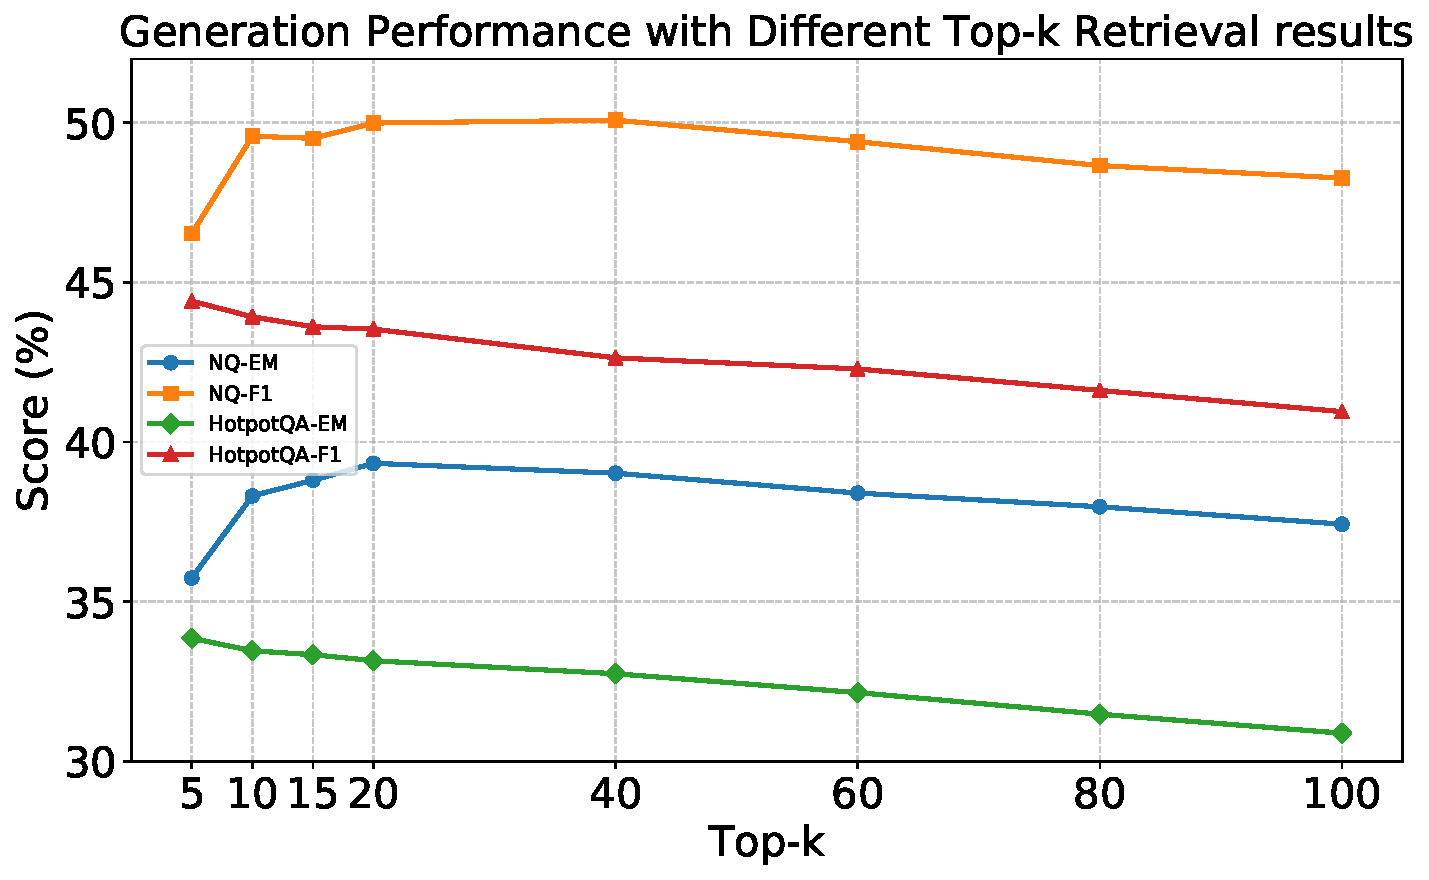
\includegraphics[width=\linewidth]{images/introduction.pdf}
%   \caption{Different answer generation performance (generator: Llama3.1-8B) directly with different Top-k retrieval results (retriever: BM25).}
%   % \Description{A woman and a girl in white dresses sit in an open car.}
%   \label{fig:original_ranked_answer}
% \end{figure}
% Ranking constitutes the core task in information retrieval (IR). Relevance serves as the foundational concept within IR \cite{mizzaro1998many}. 
% Contemporary search systems typically employ a multi-stage ranking approach \cite{guo2022semantic}, i.e., ``retrieval-then-re-ranking'' paradigm, to enhance relevance ranking performance. 
% Following initial retrieval, a re-ranker refines result ordering through fine-grained query-document interactions. 
% Conventionally, retrieval relied primarily on lexical term matching, with methods like BM25 being prominent examples \cite{robertson2009probabilistic}. More recently, dense retrieval \cite{karpukhin2020dense, xiao2022retromae, qu2020rocketqa} has become the dominant approach, encoding text into dense vectors to capture semantic similarity. Large Language Models (LLMs) have further advanced dense retrieval performance \cite{zhang2025unleashing, ma2024fine, li2024llama2vec, behnamghader2024llm2vec, zhang2025comparative}. 

% Crucially, LLMs have also revolutionized the subsequent re-ranking stage.
% Leveraging their advanced semantic understanding, LLMs offer powerful new opportunities for relevance re-ranking, particularly through zero-shot listwise re-ranking approaches \cite{sun2023chatgpt}. 
% These models can autoregressively generate entire ranked lists based on query-passage relevance \cite{pradeep2023rankvicuna, pradeep2023rankzephyr}. While larger LLMs (e.g., 32B parameters) or proprietary models often achieve superior re-ranking performance, their computational cost and latency frequently hinder real-world deployment. Consequently, a common practice distills the ranking knowledge from these powerful models into smaller, more efficient LLMs, e.g., RankVicuna \cite{pradeep2023rankvicuna}, RankZephyr \cite{pradeep2023rankzephyr}. 

% Contrasting sharply with traditional Information Retrieval (IR) objectives, which focus on ranking documents by relevance, Retrieval-Augmented Generation (RAG) operates under a fundamentally distinct paradigm. Rather than returning a ranked list of documents, RAG systems synthesize retrieved information into a single, coherent final answer. This synthesis imposes unique constraints: due to the limited input window length of the generator component (e.g., an LLM), only the top
% $k$ passages from the relevance-ranked list can be utilized as contextual evidence.

% This divergence between IR's ranking-centric output and RAG's answer-generation objective exposes critical limitations in applying conventional IR methodologies to RAG pipelines. Specifically, it raises two foundational research questions:
% \emph{Is selecting evidence solely for relevance sufficient for RAG?} 
% \emph{Is ranking indeed the optimal method for enhancing the quality of external information provided to the generator?}
% We contend that standard relevance-ranking approaches fail to address two core requirements of effective RAG:
% 1) Information Utility: RAG fundamentally depends on the functional usefulness of passages for generating accurate and comprehensive answers. Conventional relevance metrics primarily measure topical alignment (e.g., keyword overlap or semantic similarity to the query) \cite{10.1145/3731120.3744601}, which does not guarantee that a passage contains actionable evidence necessary for coherent answer synthesis. 
% % A topically relevant passage may lack specific facts, exhibit contradictions, or be redundant—undermining generator performance despite high relevance scores.
% 2) Query-Specific Adaptability: Fixed-threshold selection after re-ranking lacks per-query customization. As Figure \ref{fig:original_ranked_answer} shows, optimal document counts vary significantly across queries. 


% % Ranking is the core task in information retrieval (IR). Modern system 

% % The standard Retrieval-Augmented Generation (RAG) pipeline comprises two core components: a retriever and a generator. Conventionally, retrieval relied primarily on lexical term matching, with methods like BM25 serving as prominent examples \cite{robertson2009probabilistic}. More recently, dense retrieval \cite{karpukhin2020dense, xiao2022retromae, qu2020rocketqa} has become the prominent approach, encoding text into dense vectors to capture semantic similarity for relevance. Large Language Models (LLMs) have further significantly advanced retrieval performance \cite{zhang2025unleashing, ma2024fine, li2024llama2vec, behnamghader2024llm2vec, zhang2025comparative}, enabling the identification of a large pool of highly relevant passages. 
% % However, though modern retrievers are so effective at surfacing numerous potentially relevant passages, input window constraints and computational demands make feeding all retrieved results directly into the generator infeasible.

% % To bridge this gap, the widely adopted ``retrieval-then-re-ranking'' paradigm \cite{guo2022semantic} incorporates a critical re-ranking stage. After initial retrieval from a large corpus, a re-ranker refines the ordering of results, typically utilizing only the top-ranked passages exceeding a predefined relevance threshold for input to the generator. 

% % Leveraging their advanced semantic understanding, LLMs offer powerful new opportunities for relevance re-ranking, particularly through zero-shot listwise re-ranking approaches \cite{sun2023chatgpt}. 
% % These models can autoregressively generate entire ranked lists based on query-passage relevance \cite{pradeep2023rankvicuna, pradeep2023rankzephyr}. While larger LLMs (e.g., 32B parameters) or proprietary models often achieve superior re-ranking performance, their computational cost and latency frequently hinder real-world deployment. Consequently, a common practice distills the ranking knowledge from these powerful models into smaller, more efficient LLMs, e.g., RankVicuna \cite{pradeep2023rankvicuna}, RankZephyr \cite{pradeep2023rankzephyr}.



% % This raises two research questions: 
% % \emph{Is selecting evidence solely for relevance sufficient for RAG?} 
% % \emph{Is ranking indeed the optimal method for enhancing the quality of external information provided to the generator?}
% % We argue that relevance-ranking approaches overlook two key aspects of RAG:
% % First, RAG fundamentally requires information utility – the usefulness of retrieved passages for generating accurate and comprehensive answers. 
% % In contrast, relevance ranking primarily focuses on topical matching between passages and the query.  
% % Second, selecting passages via re-ranking followed by fixed-threshold filtering lacks query-specific adaptability. As illustrated in Figure \ref{fig:original_ranked_answer}, the optimal number of documents needed varies significantly across queries. 

% Inspired by \cite{zhang2024large, zhang2025leveraging}, we address this limitation through utility-based selection. Specifically, an LLM generates a pseudo-answer to explicitly aid itself in selecting a subset of documents from the candidate list that are most useful for answering the query. To mitigate the high inference cost of using large LLMs (e.g., 32B) for online utility-based selection, we distill the utility-based selection capability of a large LLM into a much smaller 1.7B parameter model. 
% % To overcome the LLM limitations during large-scale document candidates, we propose a forward-propagating sliding window for utility-based selection. 

% For fair comparison, we utilize the same dataset of 100k queries, sampled from the MS MARCO training set by \cite{sun2023chatgpt} for training. 
% We employ Qwen3-32B \cite{qwen3technicalreport} to generate both relevance ranking and utility-based selection outputs. 
% These outputs are then distilled into Qwen3-1.7B, yielding \rank$_{1.7B}$ (for relevance ranking) and \utility$_{1.7B}$ (for utility-based selection). 
% To evaluate RAG performance, we utilize two QA datasets from BEIR \cite{thakur2021beir}, NQ \cite{kwiatkowski2019natural}, and HotpotQA \cite{yang2018hotpotqa} on two kinds of top-100 candidate documents retrieved by two retrievers, i.e., BM25 \cite{robertson2009probabilistic} and BGE-base-en-v1.5 \cite{bge_embedding}.
% Our experimental results support our hypothesis: relevance alone is insufficient, especially on hot-pot queries; compared to ranking, selection provides a more flexible mechanism for identifying useful documents for RAG. 
% Additionally, Experiment shows the ranking performance on the BEIR benchmark \cite{thakur2021beir} of our \rank$_{1.7B}$ even is better than ChatGPT, showing superior ranking performance. Additionally, we will release the Qwen3 32B relevance ranking and utility-based selection annotations for the 100k MS MARCO dataset, providing a high-quality dataset for future research in relevance ranking and utility-based selection.



